% paper_v8.tex — workshop submission draft
% compiled from: workshop/cotknot/paper/paper_v7_5.tex
% target: NeurIPS Math-AI / ICLR SCSL / EMNLP BlackboxNLP workshop tier
\documentclass[10pt,twocolumn]{article}
\usepackage[margin=0.75in,top=0.85in,bottom=0.85in]{geometry}
\usepackage[T1]{fontenc}
\usepackage[utf8]{inputenc}
\usepackage{microtype}
\usepackage{amsmath,amssymb}
\usepackage{booktabs,tabularx,array,multirow}
\usepackage{graphicx}
\usepackage{xcolor}
\usepackage[numbers,sort&compress]{natbib}
\usepackage{hyperref}
\hypersetup{colorlinks=true,linkcolor=blue!50!black,citecolor=blue!50!black,urlcolor=blue!50!black}
\setlength{\parindent}{0.9em}
\setlength{\parskip}{0.2em}
\renewcommand{\arraystretch}{1.1}
\newcolumntype{C}{>{\centering\arraybackslash}p{1.6cm}}
\graphicspath{{../figures/}{./}}

\title{\textbf{CoT Quality Signals Are Domain-Conditioned:\\[2pt]
\large A Measurement Perspective on Math, Science, and Coding}}
\author{Yuhan Chi\\Fudan University\\\texttt{masterwuguicyh@gmail.com}}
\date{}

\begin{document}
\maketitle

\begin{abstract}
Process supervision and verifier-based reranking rest on an implicit assumption: that chain-of-thought (CoT) traces encode answer quality in a domain-neutral way. We test that assumption by using a small interpretable probe---not a new verifier---as a measurement instrument. In math and science, the signal is strong: AUC-of-AUROC reaches $0.958$ on math and $0.799$ on science, with near-lossless frozen-basis transfer across anchor positions ($\Delta$AUROC $= -0.001$ forward for math). In coding, the same feature family fails to exceed a $0.506$ token-confidence baseline (AUC-of-AUROC $0.434$), and a broader sweep over 102 coding-side scalars finds only modest alternatives. A one-hidden-layer MLP on the same feature cache preserves the ordering: $0.941 / 0.723 / 0.497$ for math/science/coding.

This is not a claim that all verifiers fail on coding. It is a narrower, better-supported claim: within this interpretable feature family, the signal \emph{stops measuring the same thing} once the domain changes. A small validation study of local state breaks is consistent with that picture---math break-like events coexist with recovery, while coding ones appear entangled with unstable execution state---but the main result stands on the full-scale comparison and does not depend on the annotation studies. Reproducible scripts and tables are in \texttt{scripts/} and \texttt{results/tables/}.
\end{abstract}

%% -------------------------------------------------------
\section{Introduction}
%% -------------------------------------------------------

There is a straightforward story about CoT-based verifiers: longer, more reflective traces tend to be more correct, so you can use trace features as a cheap quality proxy and use them to pick the best candidate among multiple rollouts. This story is well-supported for mathematical reasoning \citep{cobbe2021training,lightman2023verify,wang2024mathshepherd}. The question is whether it generalizes.

Our starting point is \emph{not} a new architecture. We use a fixed three-stage pipeline---\texttt{StandardScaler} $\to$ \texttt{TruncatedSVD} $\to$ \texttt{LogisticRegression}---trained separately on three domains: math competitions (AIME24/25, BRUMO25, HMMT25), science (GPQA), and coding (LiveCodeBench-v5). The probe is simple enough that a performance failure can be attributed to the feature family, not to model capacity.

The central finding is a measurement breakdown. When the same feature family is applied to coding traces, it not only weakens---it falls \emph{below} the baseline provided by raw token confidence. That ordering survives replacing the linear head with a nonlinear one, and it survives a broad sweep over alternative coding-side features. We interpret this as the signal no longer measuring answer quality in coding the way it does in math.

We add a small annotation study on \emph{local state breaks}---moments where the reasoning state appears to fragment or contradict itself---to probe one candidate mechanism. The study is exploratory and has real validity limits (detailed in Section~\ref{sec:limits}). It is not what drives the main finding.

%% -------------------------------------------------------
\section{Related Work}
%% -------------------------------------------------------

The core literature on CoT reasoning \citep{wei2022cot,wang2023selfconsistency} established that traces carry information beyond the final answer. Learned outcome and process reward models built on that insight \citep{cobbe2021training,lightman2023verify}, with recent extensions adding automatic step-level supervision, cross-model benchmarks, and generative verifier formulations \citep{wang2024mathshepherd,zheng2025processbench,zhang2025genrm}.

Our work sits closer to two adjacent strands. First, faithfulness analyses ask whether CoT traces mean what they appear to mean \citep{lanham2023faithfulness}; our measurement framing is in the same spirit. Second, intrinsic-self-correction work documents that reflection-like text does not always improve reasoning \citep{madaan2023selfrefine,shinn2023reflexion,huang2024selfcorrect,liu2024intrinsic}. We add a cross-domain dimension: not only is self-correction unreliable on average, but the \emph{measurability} of quality from trace features is itself domain-conditioned.

A useful analogy comes from psychometric measurement invariance \citep{vandenberg2000review}: the same instrument can measure different latent constructs in different populations. Probing work in NLP has made a related point about representation analysis \citep{belinkov2022probing}: a probe's performance depends on what the representation encodes, not just on the probe's capacity. Our result extends that logic to the verifier setting---feature families that probe correctness in math may not probe anything interpretable in coding.

%% -------------------------------------------------------
\section{Setup}
\label{sec:setup}
%% -------------------------------------------------------

\subsection{Domains and metrics}

We use three data regimes from the repository:
\textbf{Math:} 7,680 aligned runs across AIME24, AIME25, BRUMO25, and HMMT25.
\textbf{Science:} 12,672 runs from GPQA.
\textbf{Coding:} 10,688 runs from LiveCodeBench-v5.

Each run is observed at four anchor positions $a \in \{10, 40, 70, 100\}$, corresponding to the visible fraction of the trace. We report two summary metrics:
\textbf{AUROC@100\%:} final-trace discrimination.
\textbf{AUC-of-AUROC:} area under the anchor-wise AUROC curve, used as an early-stopping summary.

For cross-anchor transfer, we freeze the low-rank basis learned at a source anchor and refit only the logistic head at the target:
\[
\Delta\mathrm{AUROC} = \mathrm{AUROC}_{\text{frozen}} - \mathrm{AUROC}_{\text{task-specific}}.
\]
Values near zero mean the source basis already captures a reusable geometry.

\subsection{Feature probe}
\label{sec:probe}

The probe uses three families of cached features, intentionally kept cheap to isolate the domain effect from model capacity:

\textit{Token-confidence summaries.} \texttt{tok\_conf\_prefix} is the mean $-\log p$ over the model's top-token distribution across visible prefix tokens.

\textit{Trajectory summaries.} \texttt{traj\_continuity} is the mean Jaccard similarity between consecutive 32-token activation slices; \texttt{traj\_novelty} is mean $1-\max$ similarity to any prior slice; \texttt{traj\_reflection\_count} is the negated count of non-adjacent slice revisits exceeding similarity threshold $0.30$.

\textit{Neuron-summary.} \texttt{nc\_mean} is the prefix mean row width of the sparse rows-bank---the average number of active keys per visible slice---derived from the neuron activation cache rather than from text.

The probe is fit separately per domain. The question is not whether a universal verifier exists; it is whether the \emph{meaning} of this feature family stays stable enough within a domain and whether it changes across domains.

\subsection{Validity note on the annotation study}
\label{sec:validity}

The local-state-break annotation study (Section~\ref{sec:coding}) is exploratory. On the math side, model-assisted labeling with author review of sampled outputs yields $\kappa = 0.603$ on a 30-run human validation sample---acceptable for a pilot. On the coding side, the original GLM-assisted protocol yields $\kappa = 0.0$ on the same 30-run check (the model marks 100\% of runs positive; humans mark 6.7\%). A replacement execution-semantic protocol gives $\kappa = 0.329$ across $n = 56$ items (below threshold). These numbers mean the coding annotation study \emph{cannot} support prevalence claims or fine-grained taxonomy. We use it only for the protocol-separability question: does the same annotation logic transfer across domains?

%% -------------------------------------------------------
\section{Math and Science: Strong, Temporally Structured, Transferable}
%% -------------------------------------------------------

Table~\ref{tab:positive} shows the main result. The same probe is strong in math, respectable in science, and poor in coding.

\begin{table}[t]
\centering
\small
\begin{tabular}{lcccc}
\toprule
Domain & AoA & A@100 & Fwd $\Delta$ & Bwd $\Delta$ \\
\midrule
Math        & \textbf{.958} & \textbf{.982} & $-$.001 & $-$.006 \\
Science     & \textbf{.799} & \textbf{.841} & $-$.010 & $-$.001 \\
Coding      &  .434 &  .407 & --- & --- \\
\ \ Baseline (\texttt{tok\_conf}) & .506 & .490 & --- & --- \\
\bottomrule
\end{tabular}
\caption{Main holdout result. AoA = AUC-of-AUROC; A@100 = AUROC at 100\% anchor. Frozen-basis $\Delta$AUROC is relative to a task-specific basis at the target anchor.}
\label{tab:positive}
\end{table}

Math is not just a final-score story---it is a temporal-structure story. Across the aligned bridge table, \texttt{traj\_reflection\_count} strengthens steadily as more of the trace is revealed:
\[
\rho = -0.345\;\text{at 10\%},\quad -0.432\;\text{at 40\%},\quad -0.551\;\text{at 100\%.}
\]
Early reflection and late reflection mean different things. By the end of a trace, persistent reflection is a strong failure predictor. That is the signature of a process feature, not a surface feature.

Science is weaker and less symmetric. The forward transfer gap ($-0.010$) is noticeably larger than the backward gap ($-0.001$), suggesting that science reasoning matures later and less uniformly. The feature geometry stabilizes on a different schedule---consistent with the measurement framing: the same probe tracks a different process in a different domain.

A one-hidden-layer MLP on the same 25-dimensional feature cache under five-fold GroupKFold by problem gives $0.941 / 0.723 / 0.497$ mean anchor AUROC for math/science/coding; the 100\%-anchor AUROCs are $0.968 / 0.755 / 0.507$. Changing the classifier does not rescue coding. The cross-domain pattern is not a linear-head artifact.

%% -------------------------------------------------------
\section{Coding: The Signal Breaks Down}
\label{sec:coding}
%% -------------------------------------------------------

\subsection{Full-scale result}

On the full 10,688-run LiveCodeBench table, the best lexical proxy for self-corrective control-flow turbulence---\texttt{condition\_reversal\_per1k}---is statistically nonzero:
\[
\rho = -0.062,\qquad p = 1.15\times 10^{-10}.
\]
But the probe that works in math yields AUC-of-AUROC $0.434$ here, which is below a single-feature token-confidence baseline ($0.506$). The signal exists in the features but it does not separate correct from incorrect runs usefully.

We screen 102 interpretable coding-side scalars. The strongest negative scalar is \texttt{struct\_density} ($\rho = -0.110$, oriented AUROC $0.563$), followed by \texttt{cot\_trace\_count} ($\rho = -0.099$, AUROC $0.561$). The strongest program-structure count, \texttt{cf\_n\_ifs}, has $\rho = +0.109$ (AUROC $0.565$)---positive rather than negative. More complex code is weakly associated with more correct answers, not less. The feature sweep does not support a monotone ``more complex $\to$ more wrong'' story. Combining the top four interpretable scalars still reaches only AUROC $0.556$ under GroupKFold by problem.

This is the right place to be explicit about scope. We do not claim that all stronger verifiers fail on coding. Code-execution-aware verifiers, models with access to compiler feedback, or probes over hidden states have different information and we make no claim about them. The finding is specific: within this feature family, the measurement breaks down in coding.

\subsection{Annotation study: protocol separability}

Because the coding GLM annotation was invalid ($\kappa = 0.0$; Section~\ref{sec:validity}), we ran a replacement execution-semantic protocol on a partial LiveCodeBench subset. Table~\ref{tab:pilot} reports the expanded math pilot alongside the coding comparison.

\begin{table}[t]
\centering
\small
\begin{tabular}{lcc}
\toprule
Quantity & Value & Note \\
\midrule
Pilot-selected math runs & 256 & expanded sample \\
Usable parsed runs & 245 & after parse checks \\
Verified spans & 221 & stage-2 approved \\
Correct with break & 84/128 & rate $= 0.656$ \\
Incorrect with break & 78/117 & rate $= 0.667$ \\
Fisher exact $p$ & 0.893 & not significant \\
\midrule
\multicolumn{3}{l}{\textit{Execution-break coding protocol ($\kappa = 0.329$, $n=56$)}} \\
GLM coding human $\kappa$ & 0.0 & original protocol, invalid \\
Replacement $\kappa$ & 0.329 & below threshold \\
\bottomrule
\end{tabular}
\caption{Expanded math pilot (break prevalence) and coding annotation validity summary. Break prevalence in math is not discriminative and is not used as a main claim.}
\label{tab:pilot}
\end{table}

The prevalence of local state breaks is not discriminative in math ($p = 0.893$), so we do not use break frequency as a positive math claim. What the study does show is a geometry contrast. Inside the break-positive subset (78 correct / 63 incorrect math runs; 36 correct / 39 incorrect coding runs), the features that work in math are flat in coding:
\begin{itemize}
\item \texttt{traj\_reflection\_count} at 100\%: math $d = 1.008$ (95\% CI $[0.58, 1.48]$); coding $d = 0.013$ ($[-0.77, 0.87]$).
\item \texttt{tok\_conf\_prefix} at 100\%: math $d = 0.392$ ($[0.01, 0.82]$); coding $d = -0.284$ ($[-1.00, 0.67]$).
\item \texttt{nc\_mean} at 100\%: math $d = 0.989$ ($[0.59, 1.44]$); coding $d = -0.141$ ($[-0.94, 0.61]$).
\end{itemize}
In the expanded math pilot, the correct-minus-incorrect reflection gap is already positive at 10\% anchor (95\% CI $[1.07, 6.47]$) and grows to $[66.34, 166.10]$ at 100\%. The corresponding coding gap stays near zero at every anchor.

Figure~\ref{fig:knotprofiles} shows this directly. The $y$-axis is $\mathbb{E}[\text{feature} \mid \text{correct, break-positive}] - \mathbb{E}[\text{feature} \mid \text{incorrect, break-positive}]$. In math the gaps trend in the expected direction. In coding they stay near zero or reverse.

\begin{figure}[t]
    \centering
    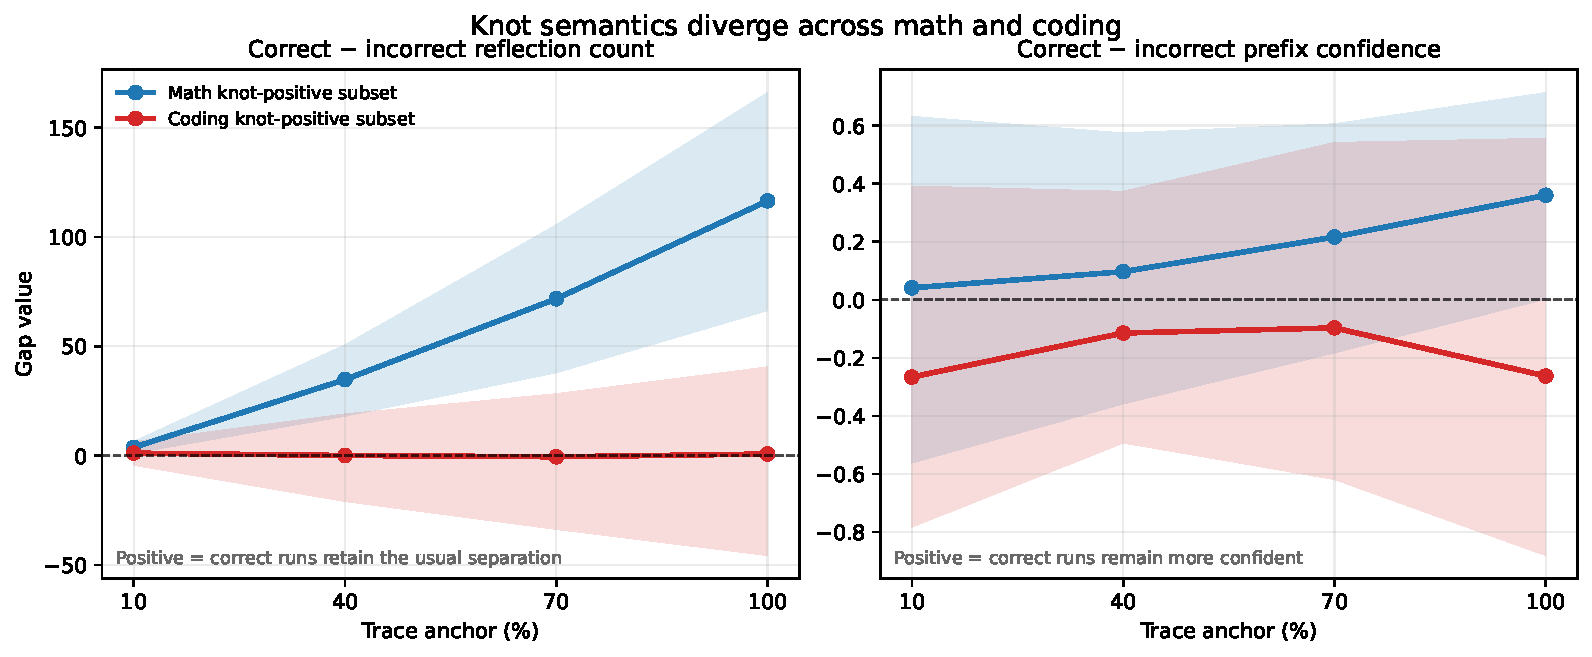
\includegraphics[width=\linewidth]{fig_knot_domain_profiles_v3.pdf}
    \caption{Feature gap inside break-positive subsets (correct minus incorrect mean, with 95\% cluster-bootstrap bands). Left: \texttt{traj\_reflection\_count}. Right: \texttt{tok\_conf\_prefix}. Math trends up; coding stays flat.}
    \label{fig:knotprofiles}
\end{figure}

A 240-run GLM-assisted coding audit gives the same reading: knot severity correlates $\rho = -0.023$ with correctness ($p = 0.723$); knot-present accuracy is $0.537$ vs.\ $0.545$ when absent; and 228 of 240 runs fall into \texttt{lost\_state}. The labels are easy to elicit but do not separate correct from incorrect runs---which is exactly what the measurement framing predicts. If the feature no longer tracks the quality object, annotating it more carefully will not fix the probe.

The timing extension uses 450 already-labeled examples (221 math, 229 coding). Onset localization succeeds in 272 cases. Among localized coding cases, all 125 fall in the first third of the trace (mean normalized onset $0.032$). Math has a longer tail: mean onset $0.109$, with 132 early / 11 middle / 4 late. The localization only succeeds on a subset, so this is suggestive rather than conclusive. But it fits: coding failures appear early as state-serialization trouble; math explicit breaks can emerge later as proof state is re-bound or contradicted.

%% -------------------------------------------------------
\section{Limitations and Conclusion}
\label{sec:limits}
%% -------------------------------------------------------

Several limits deserve direct statement.

First, the probe is deliberately simple. We do not claim state-of-the-art verifier accuracy and we do not compare against hidden-state probes, execution-aware verifiers, or generative verifier architectures. A small MLP sanity check reduces the linear-head-artifact risk but is not a baseline competition.

Second, the annotation study has real validity problems. The original coding GLM protocol yielded $\kappa = 0.0$ and is invalid for any inferential purpose. The replacement execution-semantic protocol reached $\kappa = 0.329$ ($n = 56$), which is below acceptable threshold. These numbers are disclosed here because they constrain interpretation: the coding annotation study supports a protocol-separability observation, nothing more. All main results depend on the full-scale quantitative comparison in Table~\ref{tab:positive}, not on the annotation studies.

Third, the RL regime is intentionally excluded. Verifier drift under RL fine-tuning is a real phenomenon in the repository (FPR rising from 0.982 to 0.998 across training steps), but it fits a different paper axis---regime conditioning rather than domain conditioning---and is being written separately.

The main conclusion follows from what survives all three limits:

\begin{quote}
\textbf{CoT quality signals are domain-conditioned.} In math and science, an interpretable trace probe can be strong, early-onset, and transferable across anchor positions. In coding, the same feature family drops below a token-confidence baseline and is not rescued by a broader feature sweep or a nonlinear classifier. The most plausible account is a measurement breakdown: code correctness depends on executable state evolution, whereas text and trajectory features observe only an imperfect shadow of that object.
\end{quote}

The practical implication is simple: before deploying a CoT-based verifier in a new domain, check whether the feature family measures the same thing there. Predictive performance in math does not transfer as a reliability guarantee to coding.

\paragraph{Artifacts.} Quantitative claims reproduce from \texttt{results/tables/}. Analysis scripts are in \texttt{scripts/}. The paper source is in \texttt{workshop/}.

%% -------------------------------------------------------
\bibliographystyle{plainnat}
\begin{thebibliography}{14}

\bibitem{wei2022cot}
Jason Wei et al.
\newblock Chain-of-thought prompting elicits reasoning in large language models.
\newblock In \emph{NeurIPS}, 2022.

\bibitem{wang2023selfconsistency}
Xuezhi Wang et al.
\newblock Self-consistency improves chain of thought reasoning in language models.
\newblock In \emph{ICLR}, 2023.

\bibitem{cobbe2021training}
Karl Cobbe et al.
\newblock Training verifiers to solve math word problems.
\newblock \emph{arXiv:2110.14168}, 2021.

\bibitem{lightman2023verify}
Hunter Lightman et al.
\newblock Let's verify step by step.
\newblock \emph{arXiv:2305.20050}, 2023.

\bibitem{wang2024mathshepherd}
Peiyi Wang et al.
\newblock Math-Shepherd: Verify and reinforce {LLM}s step-by-step without human annotations.
\newblock In \emph{ACL}, 2024.

\bibitem{zheng2025processbench}
Chujie Zheng et al.
\newblock ProcessBench: Identifying process errors in mathematical reasoning.
\newblock In \emph{ACL}, 2025.

\bibitem{zhang2025genrm}
Lunjun Zhang et al.
\newblock Generative verifiers: Reward modeling as next-token prediction.
\newblock In \emph{ICLR}, 2025.

\bibitem{lanham2023faithfulness}
Tamas K.\ Feher de Lanham et al.
\newblock Measuring faithfulness in chain-of-thought reasoning.
\newblock \emph{arXiv:2307.13702}, 2023.

\bibitem{liu2024intrinsic}
Dancheng Liu et al.
\newblock Large language models have intrinsic self-correction ability.
\newblock In \emph{NeurIPS}, 2024.

\bibitem{madaan2023selfrefine}
Aman Madaan et al.
\newblock Self-Refine: Iterative refinement with self-feedback.
\newblock \emph{arXiv:2303.17651}, 2023.

\bibitem{shinn2023reflexion}
Noah Shinn et al.
\newblock Reflexion: Language agents with verbal reinforcement learning.
\newblock \emph{arXiv:2303.11366}, 2023.

\bibitem{huang2024selfcorrect}
Jie Huang et al.
\newblock Large language models cannot self-correct reasoning yet.
\newblock \emph{arXiv:2310.01798}, 2023.

\bibitem{vandenberg2000review}
Robert E.\ Vandenberg and Charles E.\ Lance.
\newblock A review and synthesis of the measurement invariance literature: Suggestions, practices, and recommendations for organizational research.
\newblock \emph{Organizational Research Methods}, 3(1):4--70, 2000.

\bibitem{belinkov2022probing}
Yonatan Belinkov.
\newblock Probing classifiers: Promises, shortcomings, and advances.
\newblock \emph{Computational Linguistics}, 48(1):207--219, 2022.

\end{thebibliography}

\end{document}
